 \chapter{Energy Model}
 To optimally use the GPS receiver, we need an model that can predict the energy consumption of the system. In the first subsection, we will first analyze the data from the measurements. In the next subsection, we will present a parameter exploration for the energy model and finally, we will present the model. 
 \section{Data analysis}
 The first step in making an energy model of the GPS receiver is to analyze the data from the measurements and relating it to the theory. The theory section explains how the receiver operates between two distinct phases: acquisition and tracking. The two phases for a receiver can be modelled in a state diagram. 
 
 
\begin{figure}[H]
\centering
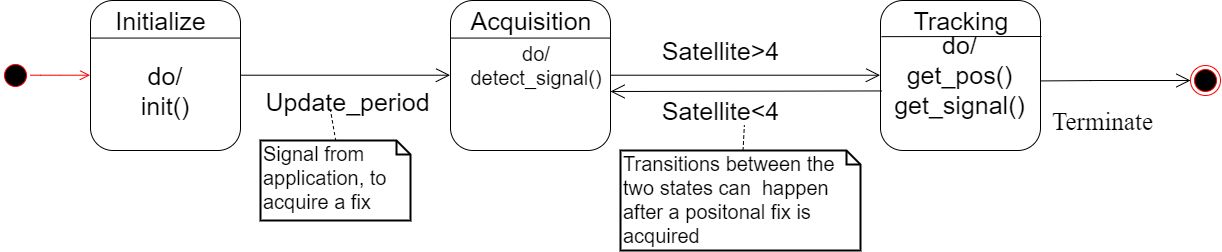
\includegraphics[width=16 cm]{Project_Report/Images/Basic_state_GPS.png}
\caption{The state diagram of a GPS receiver}
\label{fig:GPS reciever}
\end{figure}
The receiver will transition to the acquisition state once the update period is set. It will transition from the acquisition state to tracking state once it has acquired a signal from at least four satellites. 
The trigger functionality from table \ref{Table:wifioff} highlights when the receiver has a positional fix. We know from the theory, that the receiver switches to the tracking phase, once it has acquired a positional fix. The GPS receiver is therefore in tracking phase the instant the trigger is set. The trigger functionality can't however, inform about later transitions because the receiver changes phases after it has a positional fix to maintain the signal strength. A table with the data of the current consumption right before and after the trigger is set, is generated in an acquisition and a tracking column respectively. The average of each phase is calculated.  Average value of the two phases are:
\begin{itemize}
    \item Acquisition state: 80 \,mA
    \item Tracking state: 72 \,mA
\end{itemize}


Figure \ref{fig:averageacq} shows the scatter plot of the average current consumption during the acquisition phase. 
 
\begin{figure}[H]
\centering
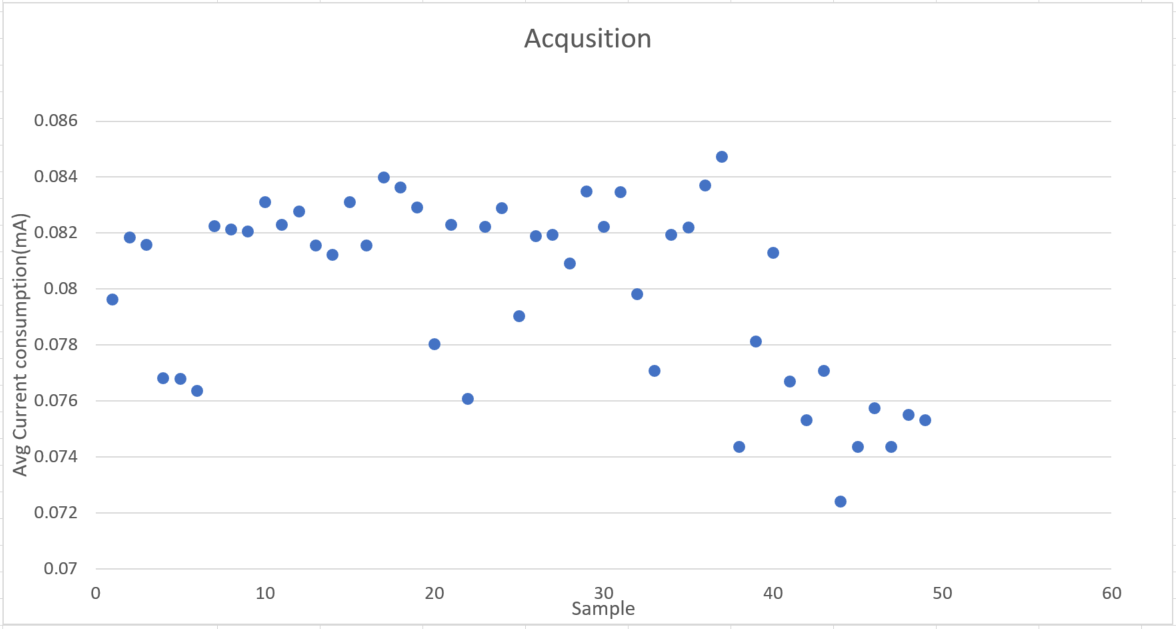
\includegraphics[width=15 cm]{Project_Report/Images/AcqusitionData.PNG}
\caption{The average values for acquisition phase in a scatter plot }
\label{fig:averageacq}
\end{figure}

Figure \ref{fig:averagetrack} shows the scatter plot of the average current consumption during the tracking phase.

\begin{figure}[H]
\centering
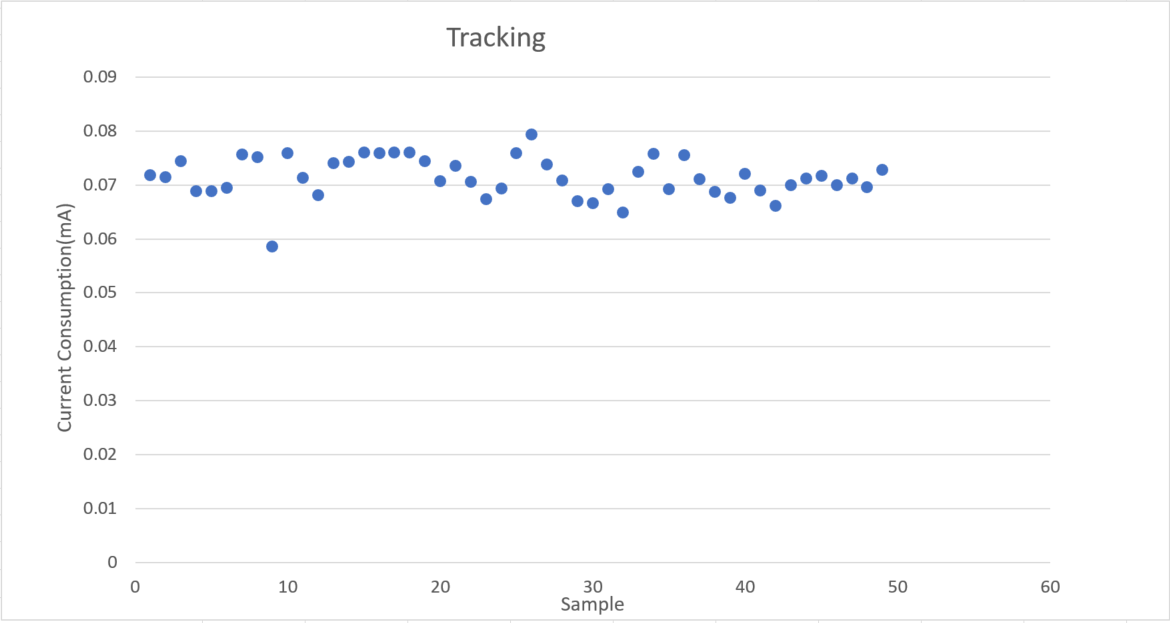
\includegraphics[width=15 cm]{Project_Report/Images/trackingData.PNG}
\caption{The average values for tracking phase in a scatter plot }
\label{fig:averagetrack}
\end{figure}
 
The scatter plots shows how the current consumption is decreasing in the later samples for both phases. The schematics from figure \ref{fig:LoPy_Schematic} shows that the LoPy is using a LiPo battery for voltage supply. Rechargeable batteries  tend to have a discharge curve, which means that the battery voltage changes during discharge. This affect might be the cause of the deviating voltage values in the later measurements. 

The average values are compared with the features from the datasheet \cite{L76}. The datasheet specifies that it should be a 7 \,mA difference between the acquisition and tracking phase. This seems to validate the measurements, which shows a decreasing in current consumption from 80 \,mA to 72 \,mA after a positional fix.   
\section{Parameter exploration}
The next step in developing an model is to determine which parameters that the model should be dependent on. The parameters in the model will determine the accuracy and abstraction level of the model. We decided to make a simple model with few parameters because of the limited project time.

Based on the theory, we know that the time used in the acquisition state varies accordingly to the validity of the satellite data and signal strength to the satellite. To develop a simple model, we do an optimistic assumption that the time used in acquisition is only dependent on satellite data, and therefore equal to either 35 \,s, 30 \,s or 1 \,s from the specification\cite{L76}. Validity of satellite data is for this reason a parameter for the model. We also assume that the receiver doesn't switch between the acquisition state and tracking state after acquiring a fix, even if it's kept in tracking state. 

Another parameter is the enabling of deepsleep. The receiver can either be kept in tracking phase continuously or it can be put to deepsleep between update periods. Deepsleep introduces an overhead which consists of initializing the receiver and acquiring signal strength between each updating period. It may therefore exist a scenario where it's better to have a continuously fix in tracking, instead of using deepsleep. 

The state diagram in figure \ref{fig:GPS energymodel} is an extension of the general state diagram from figure \ref{fig:GPS reciever}. The state diagram is extended with a deepsleep state and an internal transition if the receiver is kept in tracking state. Timeouts are used for setting time constraints for acquiring a positional fix. 

\begin{figure}[h]
\centering
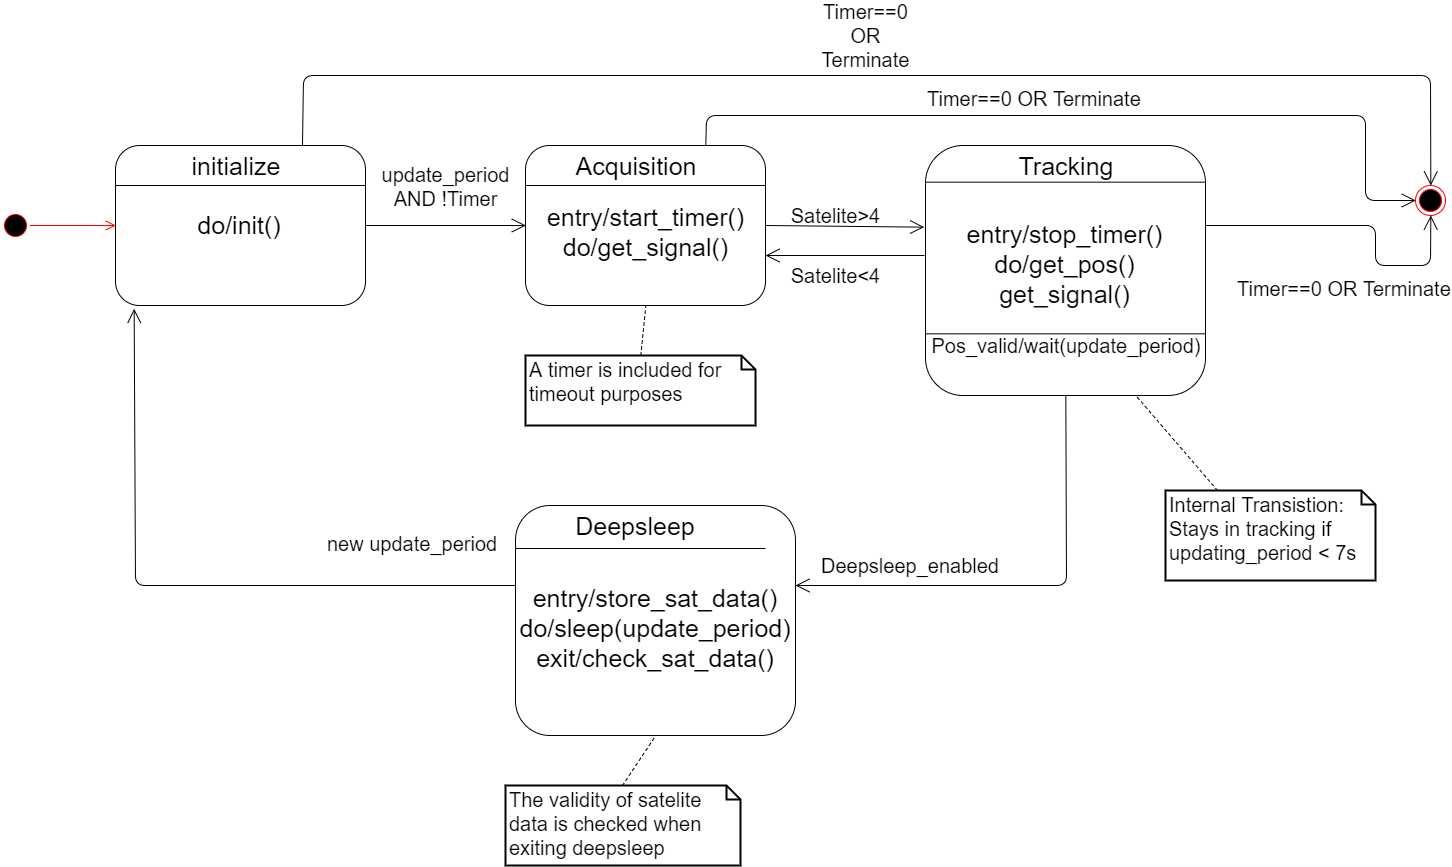
\includegraphics[width=15 cm]{Project_Report/Images/Energymodel.png}
\caption{The state diagram which represent the energy model}
\label{fig:GPS energymodel}
\end{figure}

\section{The model}
We can derive a prediction of the energy cost of acquiring a fix, by using the state diagram from \ref{fig:GPS energymodel}. The prediction will highlight which update period that is beneficial for having an optimal energy strategy. 
 
The Python script in appendix \ref{Appendix:make_energy_model.py} use the method that is derived in this subsection to predict the energy consumption over a range of update periods and durations. An update period is defined as the time from the microcontroller sends a positional request until the next request. The energy consumption over an update period is:
\begin{equation}
E_{period} = P_{period}*T_{period}
\end{equation}
\label{equation:general}
During an update period, the microcontroller transitions between the states in figure \ref{fig:GPS energymodel}. The total energy consumption $E_{fixperiod}$ can therefore be written as the sum of the energy of each state:

\begin{equation}
E_{period} = P_{Initialize}*T_{Initialize} + P_{Acquisition}*T_{Acquisition} + P_{Tracking}*T_{Tracking} + P_{Deepsleep}*T_{Deepsleep}
\end{equation}
\label{equation:energyperiod}

If the microcontroller is kept in tracking state, the initial energy used in initialize, acquisition and deepsleep is omitted. We omit the initial energy used in initialize and acquisition for the first fix during an update period of 1 \,s, because it becomes insignificant over a long duration. 
\begin{equation}
E_{Period = 1 \,s} = P_{Tracking}*T_{Tracking}
\end{equation}
\label{equation:1s}


The time used in deepsleep during an update period is dependent on the overhead of waking the microcontroller from deepsleep and acquiring a fix:

\begin{equation}
T_{Deepsleep} = T_{Updateperiod} - T_{Initialize} - T_{Acquisition} - T_{Tracking}
\end{equation}
\label{equation:energydeepsleep}
$T_ {Acquisition}$ depends on the validity of satellite data which is given by the update period. The total energy consumption over a duration t is given by the energy consumption of a fix period multiplied by the number of periods during the total duration t:

\begin{equation}
 E_{total} = E_{Updateperiod}* \frac{t}{Updateperiod}
\end{equation}
\label{equation:energytotal}

 We can use the average values from the previous subsection to calculate the power consumption for each state. This is shown in table  \ref{Table:data for the energy model}. The power is also plotted in a pie diagram in figure \ref{fig:powerconsumption}
\begin{table}[h!]
\begin{center}
 \begin{tabular}{||c c||} 
 \hline
  State &  Power(W) \\ [0.5ex] 
 \hline\hline
  Initialize & 0.32099 \\ 
 \hline
 Acquisition & 0.2576 \\
 \hline
 Tracking & 0.2324 \\
 \hline
 Deepsleep & 0.0105 \\
 [1ex]
 \hline
\end{tabular}
\end{center}
\caption{Power consumption of each state}
\label{Table:data for the energy model}
\end{table}

\begin{figure}[H]
\centering
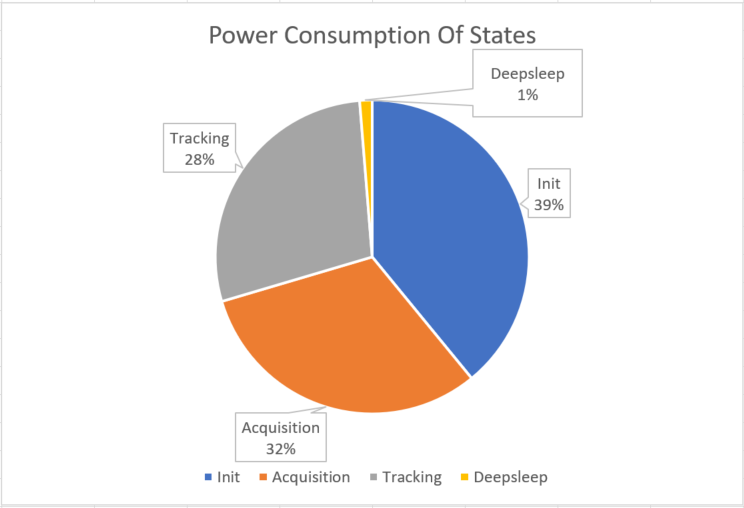
\includegraphics[height=7.5cm]{Project_Report/Images/Power.PNG}
\caption{The pie diagram of the power in table \ref{Table:data for the energy model}}
\label{fig:powerconsumption}
\end{figure}

The pie diagram shows how the majority of the power is associated with the initializing of the microcontroller. The second biggest contribution to power consumption is the acquisition state, followed by the tracking state. The power consumption in deepsleep is insignificant compared to the other states, which further encourage the use of deepsleep as a power saving strategy. The energy consumption over 1 year with a range of update periods included in table \ref{Table:energy}. The table is derived by using equation 6.5


\begin{table}[h!]
\begin{center}
 \begin{tabular}{||c c||} 
 \hline
 Energy Consumption & \\
 \hline
  Update Period & Duration = 1 year \\[0.5ex] 
 \hline\hline
  1 \,s & 7329470.97 \,J \\ 
 \hline
  7 \,s & 9485627.84 \,J \\
  \hline
  8 \,s & 8341511.51 \,J \\
  \hline
  9 \,s & 7451643.26 \,J \\
  \hline
  10 \,s & 6739748.65 \,J \\
 \hline
  60 \,s & 1400539.13 \,J \\
 \hline
  1800 \,s & 368291.96 \,J \\
  \hline
  3600 \,s & 350494.59 \,J \\
  \hline
  14399 \,s & 337146.88 \,J \\
  \hline
  14400 \,s & 352836.73 \,J \\
  \hline
  15551700 \,s & 332715.87 \,J \\
  \hline
  15552000 \,s & 332718.38 \,J \\[1ex]
 \hline
\end{tabular}
\end{center}
\caption{Table displaying the energy consumption over different durations and update periods}
\label{Table:energy}
\end{table}


\section{Energy Analysis}

The pie diagram from \ref{fig:powerconsumption} doesn't identify the energy demand of each state. The energy consumption of a state depends on the time that it's active. We know from equation 6.5 that it's only the time used in acquisition and deepsleep that varies. All the other times in our model is static. The time used in acquisition is an important factor for energy consumption. As explained in the theory chapter, the receiver can be in of three scenarios: 

\begin{itemize}
    \item Valid Ephemeris \& valid Almanac: Time used in acquisition: 1\,s. This is the scenario when the update period is in the range [1,14399]\,s. This scenario is equal to a Hot start.
    \item Invalid Ephemeris \& valid Almanac: Time used in acquisition: 30\,s. This is the scenario when the update period is in the range [14400,15551700]\,s. This scenario is equal to a Warm start.
    \item Invalid Ephemeris \& invalid Almanac: Time used in acquisition: 35\,s. This is the scenario when the update period is in the range [15551700, $\infty$ ]\,s. This scenario is equal to a Cold start.
\end{itemize}

We suspect that the energy consumption of each state will vary for each scenario, since the time in acquisition state varies. 

\subsection{Valid Ephemeris \& valid Almanac}

Figure \ref{fig:firstcase} shows the energy consumption over a duration of 1 year when the update period is 14399 \,s. The pie diagram shows the contribution from each state to the energy consumption. 

\begin{figure}[H]
\centering
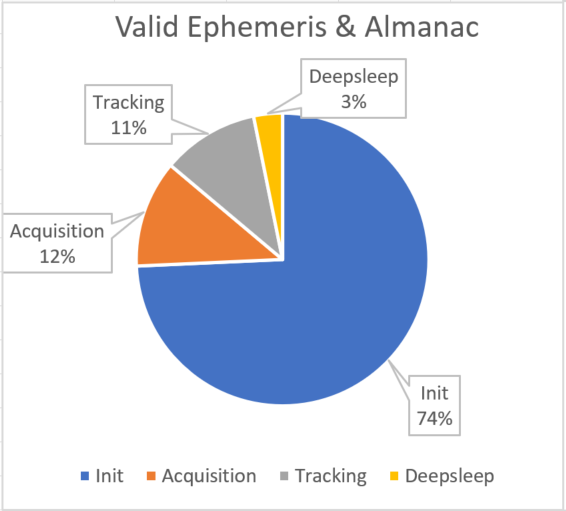
\includegraphics[height=7.5cm]{Project_Report/Images/Allvalid.PNG}
\caption{The energy consumption over 1 year with an update period of 14399 seconds}
\label{fig:firstcase}
\end{figure}

The GPS receiver uses only 1 \,s in the acquisition state because of the validity of the satellite data. This makes the initializing state, the main factor for the energy consumption. The receiver spends a small amount of time in deepsleep because of the high update frequency. This makes the deepsleep an insignificant contributor to the energy consumption. 

\subsection{Invalid Ephemeris \& valid Almanac}
Figure \ref{fig:secondcase} shows the energy contribution over 1 year for each state when the update period is 14400 \,s. An update period of [14400,15551700] \,s will make the Ephemeris invalid.

\begin{figure}[H]
\centering
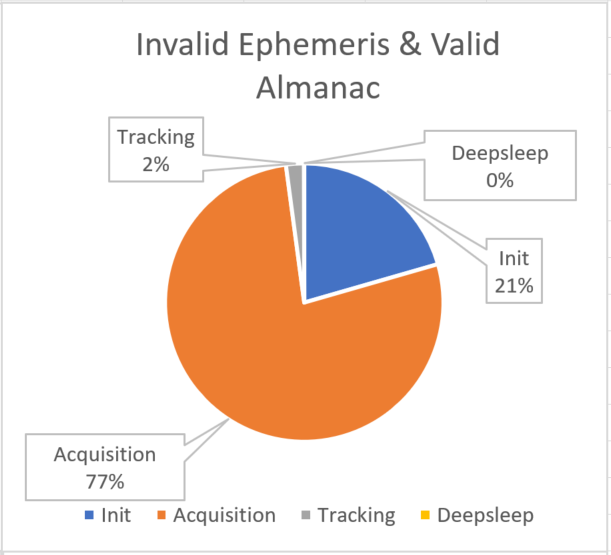
\includegraphics[height=7.5cm]{Project_Report/Images/invalidvalid.PNG}
\caption{The energy consumption over 1 year with an update period of 14400 seconds}
\label{fig:secondcase}
\end{figure}

Comparing figure \ref{fig:firstcase} with figure \ref{fig:secondcase}, we can see that the major energy consumer isn't the initialization state but the acquisition state. This is because of the added time penalty of waiting 30 \,s instead of 1 \,s in acquisition state. The added time penalty comes from time used in acquisition to download a valid Ephemeris. The update frequency is high, which makes the receiver spend a small time in deepsleep. This makes deepsleep a small part of the energy consumption.  

\subsection{Invalid Ephemeris \& invalid Almanac}

The energy consumption of each state when both the Ephemeris and Almanac is invalid is show in figure \ref{fig:thirdcase}.

\begin{figure}[H]
\centering
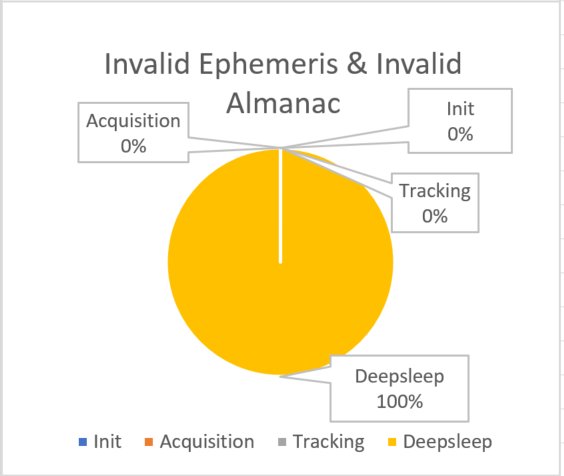
\includegraphics[height=7.5cm]{Project_Report/Images/invalidinvalid.PNG}
\caption{The energy consumption over 1 year with an update period of 15551700 seconds}
\label{fig:thirdcase}
\end{figure}

 Both the Ephemeris and Almanac is invalid when an update period of 15551700 \,s (180 days) is used. The receiver has to spend 35 \,s in the acquisition state to download the valid satellite data. The pie diagram in figure \ref{fig:thirdcase} is different from figure \ref{fig:firstcase} and figure \ref{fig:secondcase}, in that the major energy consumption is from deepsleep. This is because of the low update frequency which cause the system to spend the majority of its time in deepsleep. A longer update period will therefore use less energy but give a coarser positional fix over a specific duration. 

\newpage